\tikzstyle{vertex} = [draw=black,fill=black,circle,inner sep=0pt,minimum size=3pt]
\tikzstyle{chosen} = [draw=black,fill=red,circle,inner sep=0pt,minimum size=5pt]
\tikzstyle{edgeI} = [draw=black]
\tikzstyle{edgeTree} = [draw=black]
\tikzstyle{comp} = [draw=black,fill=white,circle,inner sep=0pt,minimum size=20pt]
\tikzstyle{cliqueS} = [blue, line width=2pt, fill=blue!30]
\tikzstyle{cliqueT} = [green, line width=2pt, fill=green!30]

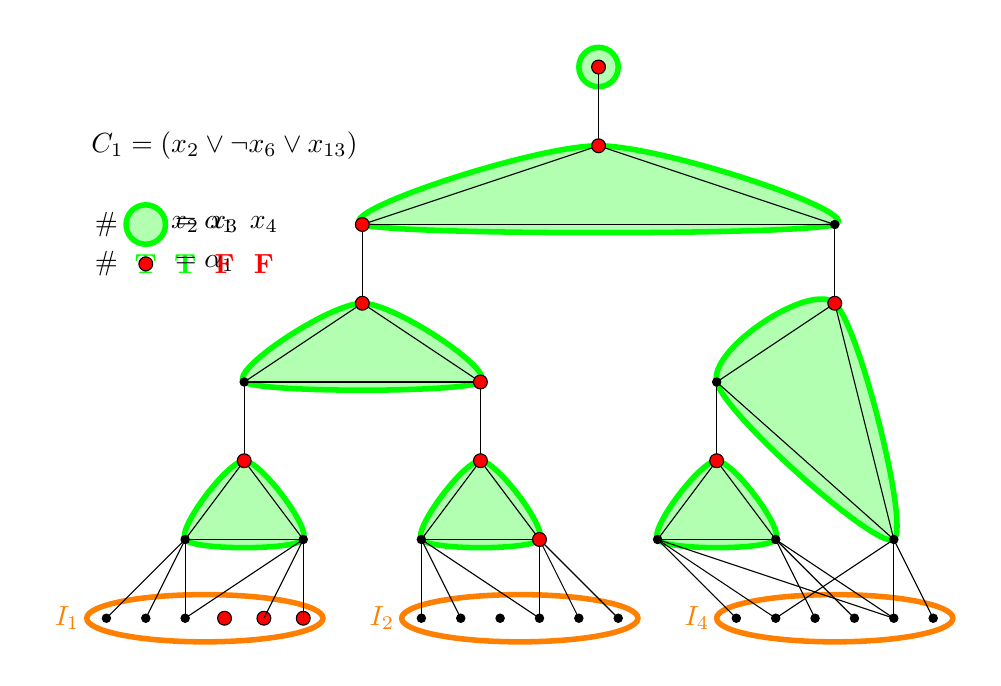
\begin{tikzpicture}[scale=0.5]
    \path (-1,-1) -- (23,-1) -- (23,15) -- (-1,15) -- cycle;

    \node<-23> at (4, 12) {$C_1 = (x_2 \lor \lnot x_6 \lor x_{13})$};

    \foreach \x in {1,...,4}{
        \coordinate (X\x) at (\x + 1, 10);
        \coordinate (VX\x) at (\x + 1, 9);
        \node<3-5> at (X\x) {$x_\x$};
    }

    \node<3-5> at (VX1) {\textbf{\color{green}T}};
    \node<3-5> at (VX2) {\textbf{\color{green}T}};
    \node<3-5> at (VX3) {\textbf{\color{red}F}};
    \node<3-5> at (VX4) {\textbf{\color{red}F}};

    \foreach \n in {0,...,2}{
        \foreach \x in {1,...,6}{
            \coordinate (N\n\x) at (8*\n + \x, 0);
            \node<2->[style=vertex] at (N\n\x) {};
        }
    }

    \draw<2-> [orange, line width=2pt] (3.5, 0) ellipse (3cm and .6cm);
    \node<2-> at (0,0) {\color{orange}$I_1$};
    \draw<2-> [orange, line width=2pt] (11.5, 0) ellipse (3cm and .6cm);
    \node<2-> at (8,0) {\color{orange}$I_2$};
    \draw<2-> [orange, line width=2pt] (19.5, 0) ellipse (3cm and .6cm);
    \node<2-> at (16,0) {\color{orange}$I_4$};

    \foreach \x in {1,...,7}{
        \coordinate (T\x) at (3*\x, 2);
    }
    \foreach \x in {1,...,3}{
        \coordinate (T1\x) at (6*\x - 1.5, 4);
        \coordinate (T2\x) at (6*\x - 1.5, 6);
    }
    \foreach \x in {1,...,2}{
        \coordinate(T3\x) at (12*\x - 4.5, 8);
        \coordinate(T4\x) at (12*\x - 4.5, 10);
    }
    \coordinate (T51) at (13.5, 12);
    \coordinate (T61) at (13.5, 14);

    % \draw<15> [style=cliqueS] ($(T11)!0.5!(T21)$) ellipse (.6cm and 1.5cm);
    % \draw<15> [style=cliqueS] ($(T12)!0.5!(T22)$) ellipse (.6cm and 1.5cm);
    % \draw<15> [style=cliqueS] ($(T13)!0.5!(T23)$) ellipse (.6cm and 1.5cm);
    % \draw<15> [style=cliqueS] ($(T31)!0.5!(T41)$) ellipse (.6cm and 1.5cm);
    % \draw<15> [style=cliqueS] ($(T32)!0.5!(T42)$) ellipse (.6cm and 1.5cm);
    % \draw<15> [style=cliqueS] ($(T51)!0.5!(T61)$) ellipse (.6cm and 1.5cm);
    
    \draw<15-> [style=cliqueT] plot [smooth cycle] coordinates {(T1) (T2) (T11)};
    \draw<15-> [style=cliqueT] plot [smooth cycle] coordinates {(T3) (T4) (T12)};
    \draw<15-> [style=cliqueT] plot [smooth cycle] coordinates {(T5) (T6) (T13)};
    \draw<15-> [style=cliqueT] plot [smooth cycle] coordinates {(T21) (T22) (T31)};
    \draw<15-> [style=cliqueT] plot [smooth cycle] coordinates {(T7) (T23) (T32)};
    \draw<15-> [style=cliqueT] plot [smooth cycle] coordinates {(T41) (T42) (T51)};
    \draw<15-> [style=cliqueT] (T61) ellipse (.5cm and .5cm);

    \node<15-23> at (1, 10) {\#};
    \draw<15-23> [style=cliqueT] (2,10) ellipse (.5cm and .5cm);
    \node<15-23> at (3.5, 10) {$= \alpha_1$};

    \node<4->[style=vertex] at (T1) {};
    \foreach \x in {4,5,6} {
        \node<3-5>[style=chosen] at (N0\x) {};
    }
    \foreach \x in {1,2,3} {
        \draw<5->[style=edgeI] (N0\x) -- (T1);
    }
    \node<6->[style=vertex] at (T2) {};
    \foreach \x in {3,5,6} {
        \draw<6->[style=edgeI] (N0\x) -- (T2);
    }
    \node<6->[style=vertex] at (T3) {};
    \foreach \x in {1,2,4} {
        \draw<6->[style=edgeI] (N1\x) -- (T3);
    }
    \node<6->[style=vertex] at (T4) {};
    \foreach \x in {4,5,6} {
        \draw<6->[style=edgeI] (N1\x) -- (T4);
    }
    \node<6->[style=vertex] at (T5) {};
    \foreach \x in {1,2,5} {
        \draw<6->[style=edgeI] (N2\x) -- (T5);
    }
    \node<6->[style=vertex] at (T6) {};
    \foreach \x in {3,4,5} {
        \draw<6->[style=edgeI] (N2\x) -- (T6);
    }
    \node<6->[style=vertex] at (T7) {};
    \foreach \x in {2,5,6} {
        \draw<6->[style=edgeI] (N2\x) -- (T7);
    }

    \node<8-> [style=vertex] at (T11) {};
    \node<9-> [style=vertex] at (T21) {};
    \draw<7-> [style=edgeTree] (T1) -- (T2);
    \draw<8-> [style=edgeTree] (T1) -- (T11);
    \draw<8-> [style=edgeTree] (T2) -- (T11);
    \draw<9-> [style=edgeTree] (T11) -- (T21);

    \node<10-> [style=vertex] at (T12) {};
    \node<10-> [style=vertex] at (T22) {};
    \draw<10-> [style=edgeTree] (T3) -- (T4);
    \draw<10-> [style=edgeTree] (T3) -- (T12);
    \draw<10-> [style=edgeTree] (T4) -- (T12);
    \draw<10-> [style=edgeTree] (T12) -- (T22);

    \node<11-> [style=vertex] at (T13) {};
    \node<11-> [style=vertex] at (T23) {};
    \draw<11-> [style=edgeTree] (T5) -- (T6);
    \draw<11-> [style=edgeTree] (T5) -- (T13);
    \draw<11-> [style=edgeTree] (T6) -- (T13);
    \draw<11-> [style=edgeTree] (T13) -- (T23);

    \node<12-> [style=vertex] at (T32) {};
    \node<12-> [style=vertex] at (T42) {};
    \draw<12-> [style=edgeTree] (T7) -- (T23);
    \draw<12-> [style=edgeTree] (T7) -- (T32);
    \draw<12-> [style=edgeTree] (T23) -- (T32);
    \draw<12-> [style=edgeTree] (T32) -- (T42);

    \node<13-> [style=vertex] at (T31) {};
    \node<13-> [style=vertex] at (T41) {};
    \draw<13-> [style=edgeTree] (T21) -- (T22);
    \draw<13-> [style=edgeTree] (T21) -- (T31);
    \draw<13-> [style=edgeTree] (T22) -- (T31);
    \draw<13-> [style=edgeTree] (T31) -- (T41);

    \node<14-> [style=vertex] at (T51) {};
    \node<14-> [style=vertex] at (T61) {};
    \draw<14-> [style=edgeTree] (T41) -- (T42);
    \draw<14-> [style=edgeTree] (T41) -- (T51);
    \draw<14-> [style=edgeTree] (T42) -- (T51);
    \draw<14-> [style=edgeTree] (T51) -- (T61);

    \node<16-23>[style=chosen] at (T11) {};
    \node<16-18>[style=chosen] at (T12) {};
    \node<16-23>[style=chosen] at (T13) {};
    \node<17-19>[style=chosen] at (T31) {};
    \node<17-23>[style=chosen] at (T32) {};
    \node<18-20>[style=chosen] at (T51) {};

    \node<19-23>[style=chosen] at (T4) {};
    \node<20-23>[style=chosen] at (T22) {};
    \node<21-23>[style=chosen] at (T41) {};
    \node<22-23>[style=chosen] at (T61) {};

    \node<23>  at (1, 9) {\#};
    \node<23> [style=chosen] at (2, 9) {};
    \node<23>  at (3.5, 9) {$= \alpha_1$};
\end{tikzpicture}